\section{Ablation, baselines, and robustness}\label{app:ablation}

\subsection{Splitting chains on a basin map}\label{sec:chains}
Figure~\ref{fig:suschains} shows how the chains of the splitting arm of section~\ref{sec:sus} are distributed over the basin map of a Jiang map in the first two levels.

\begin{figure}[tbhp]
\centering
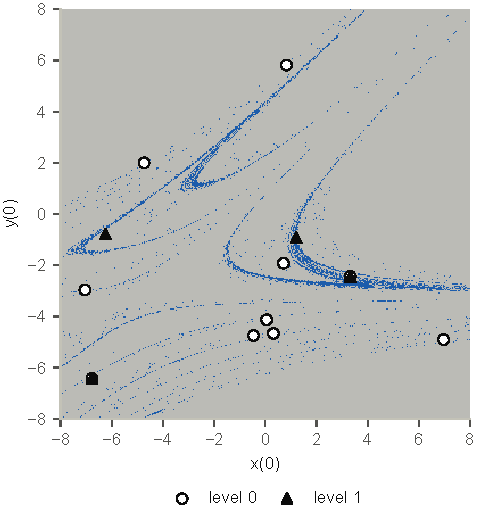
\includegraphics[width=0.62\textwidth]{figures/fig38_sus_chains.pdf}
\caption{Splitting chains on the basin map of the Jiang map NF~I~e (gray: escape; blue: basin of the chaotic attractor): seeds of levels 0 (open circles) and 1 (triangles). Already at the second level, the chains sit on thin ``tongues'' of the basin, since the escape step is larger near their edges; the target is found after 90 integrations. Seeds that coincide are drawn once.}
\label{fig:suschains}
\end{figure}

\subsection{Ablation and baselines}\label{sec:ablation_main}
Table~\ref{tab:gainsfull} gives the gains of all strategies on the rare targets of levels A and B with their bootstrap intervals.

\begin{table}[tbhp]
\centering
\caption{Full version of Table~\ref{tab:gains}: gain factors $G_{0.9}=N^0_{0.9}/N_{0.9}$ with 95\% bootstrap intervals ($R=100$); $p$ is the combined measure of the two symmetric attractors where there are two. DE: differential evolution with Zelinka's cost function; AL: active learning with the 20\% uniform share; +NC: portfolio with nullcline sampling. Bold: values whose lower interval bound exceeds 1; the intervals are given under the values. ``---'': the variant was not run. For the Jiang maps, the individual cases are given without intervals.}
\label{tab:gainsfull}
\footnotesize
\setlength{\tabcolsep}{4pt}

\begin{tabular}{lrrrrrrr}
\toprule
System & $p$ & $N^0_{0.9}$ & DE & Splitting & AL & Portfolio & +NC \\
\midrule
Chua I & 0.035 & 66 & 0.60 & 1.20 & 1.23 & 1.24 & \textbf{4.42} \\
 &  &  & \ci{0.43}{0.99} & \ci{0.92}{1.77} & \ci{0.95}{1.74} & \ci{0.94}{1.77} & \ci{3.27}{6.47} \\[1pt]
Chua II & 0.0027 & 818 & 0.84 & \textbf{5.05} & \textbf{3.16} & \textbf{7.36} & \textbf{7.64} \\
 &  &  & \ci{0.67}{1.32} & \ci{4.13}{7.07} & \ci{2.58}{4.90} & \ci{6.09}{10.2} & \ci{5.98}{11.8} \\[1pt]
SE11 & 0.0079 & 317 & 0.95 & \textbf{2.53} & \textbf{3.62} & \textbf{3.10} & \textbf{3.56} \\
 &  &  & \ci{0.72}{1.07} & \ci{1.95}{2.86} & \ci{2.63}{4.16} & \ci{2.46}{3.70} & \ci{2.71}{4.31} \\[1pt]
LE1 & 0.0016 & 1617 & 1.31 & \textbf{8.29} & 0.48 & \textbf{6.24} & \textbf{4.62} \\
 &  &  & \ci{0.94}{2.08} & \ci{6.35}{12.3} & \ci{0.32}{1.49} & \ci{3.76}{10.0} & \ci{3.03}{10.7} \\[1pt]
Jafari, cycle & 0.009 & 219 & 0.29 & 0.29 & 0.88 & 0.43 & 0.32 \\
 &  &  & \ci{0.19}{0.50} & \ci{0.19}{0.53} & \ci{0.66}{1.41} & \ci{0.29}{0.78} & \ci{0.25}{0.50} \\[1pt]
Huynh 2019 & 0.0091 & 221 & 0.45 & 1.36 & 0.82 & \textbf{1.40} & --- \\
 &  &  & \ci{0.34}{0.85} & \ci{0.79}{2.42} & \ci{0.57}{1.72} & \ci{1.16}{2.54} &  \\[1pt]
Jafari, chaos & $(2$--$5)\times10^{-4}$ & 5265 & 0.23 & 0.22 & 1.08 & 0.42 & 0.27 \\
 &  &  & \ci{0.16}{0.28} & \ci{0.15}{0.28} & \ci{0.57}{1.40} & \ci{0.29}{0.58} & \ci{0.16}{0.32} \\[1pt]
\midrule
Jiang NF I e & 0.028--0.039 & 109 & 0.83 & 1.52 & 1.02 & 1.46 & --- \\
\quad NF I f & & 86 & 0.90 & 1.23 & 1.51 & 1.49 & --- \\
\quad NF I g & & 71 & 1.00 & 1.08 & 1.15 & 1.23 & --- \\
Jiang SF I a & 0.065 & 36 & 0.75 & 1.00 & 1.00 & 1.00 & --- \\
\quad SF I b & & 33 & 0.92 & 1.00 & 1.00 & 1.00 & --- \\
\bottomrule
\end{tabular}

\end{table}


\textbf{Ablation.} The contributions of the components are shown in Figure~\ref{fig:ablation}. On Chua~II, the arms add up: the portfolio gives 7.4 times, versus 5.1 for splitting and 3.2 for active learning. On LE1, the active-learning arm hurts, and the gain of the portfolio is provided by the splitting arm. Without the uniform share, the portfolio is not faster (Chua~II: 7.0; SE11: 3.1; LE1: 5.1) and loses where there is no signal (Jafari cycle: 0.27 against 0.43). On LE1, the lower interval bound for $G$ without the uniform share is 1.59, whereas for the portfolio with $\theta=0.2$, it is 3.76. Multidimensional ``rarity'' as a reaction coordinate produces heavy tails: the chains get stuck in atypical but nontarget regions, for example, in the basin of an equilibrium inside the D2 ball. The escape step as a coordinate is equivalent to $\xi$ everywhere except Chua~II, where all trajectories are bounded and it gives 1.04 against 5.05. Two earlier strategies were also tested ($R=20$): adaptive multilevel splitting driven by the novelty of the asymptotic fingerprint finds the target on Chua~II in only 55\% of runs, and MAP-Elites with the fingerprint as behavior descriptor has a median 5.6 times better than uniform sampling but a heavy tail, $G=0.36$. Such tails are what the uniform share of the portfolio removes.

\begin{figure}[tbhp]
\centering
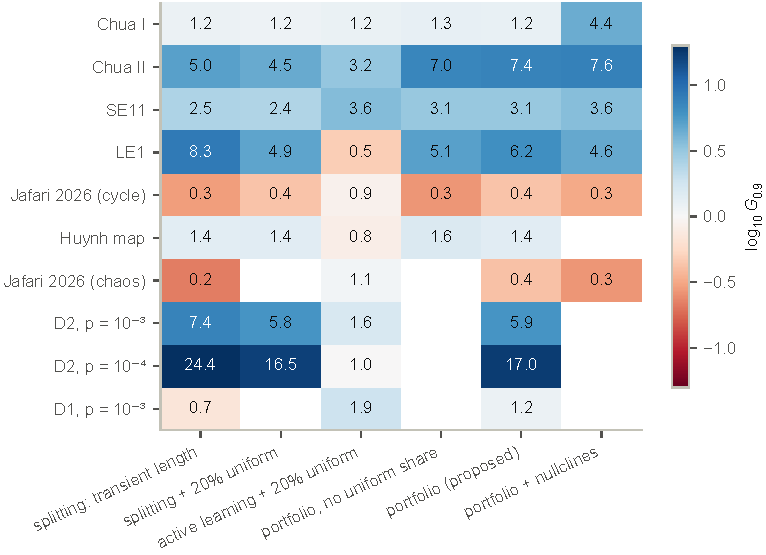
\includegraphics[width=\textwidth]{figures/fig25_ablation.pdf}
\caption{Ablation: $G_{0.9}$ of the variants of the method relative to uniform sampling ($R=100$; color: $\log_{10}G$; empty cells: the variant was not run). Rows: systems of levels A and B and synthetic families; columns: splitting alone and with a uniform share, active learning with a uniform share, the portfolio without a uniform share, the portfolio, and the portfolio with nullclines. Columns 1, 3, 5, and 6 repeat Table~\ref{tab:gains}; the new information is in columns 2 and 4 and in the D1 and D2 rows.}
\label{fig:ablation}
\end{figure}

% Differential-evolution baseline: exact description of the implementation
% (src/hsearch/search/strategies.py, class DEZelinka; harness in src/hsearch/search/harness.py;
% configuration in experiments/e50_batch_runner.py and e20_search_benchmark.py).
% One paragraph, no table; intended for the appendix.

\textbf{Differential-evolution baseline.} The baseline is differential evolution over initial conditions with the cost function of Ref.~\cite{Zelinka2016}, in the variant DE/rand/1/bin used there. The population has $N_P=25$ members (half of the initial sample $n_0=50$ of the other strategies, but not fewer than 10), the differential weight is $F=0.9$, and the crossover probability is $C_R=0.3$, the values of Ref.~\cite{Zelinka2016}. The initial population is drawn uniformly from the region $B$ and consists of the first 25 points of the uniform stream of the run, so that it coincides with the first 25 points of uniform sampling (common random numbers). In every generation, for each member $x_i$, three other members $x_{r_1}$, $x_{r_2}$, $x_{r_3}$, distinct from one another and from $x_i$, are drawn without replacement; the mutant is $v=x_{r_3}+F\,(x_{r_1}-x_{r_2})$; the trial $u_i$ takes each coordinate from $v$ with probability $C_R$ and from $x_i$ otherwise, with one randomly chosen coordinate always taken from $v$; and $u_i$ is clipped to $B$ coordinate by coordinate. The 25 trials of a generation form one batch and are integrated with the full protocol ($T_{\rm tr}+T_{\rm obs}$ of Table~\ref{tab:integration}); $u_i$ replaces $x_i$ if its cost does not exceed that of $x_i$. The cost is computed from the trajectory fingerprint alone. Let $r_{\max}$ be the maximum of the Euclidean norm of the state over the observation window $T_{\rm obs}$ (after the transient $T_{\rm tr}$); the cost is 0 if $d_{\rm lo}\le r_{\max}\le d_{\rm hi}$ and $r_{\max}$ otherwise, and it is $10^6$ for a trajectory that escapes beyond $R_{\rm esc}$ or produces a nonfinite state at any time. This is the function of Ref.~\cite{Zelinka2016}, where the maximum is taken over the last 50 time units of a run of length 200 and the interval $[d_{\rm lo},d_{\rm hi}]=[3,11]$ was chosen empirically for the hidden attractor of the Chua circuit. The pair $(3,11)$ remains the default in the implementation but is not used in the benchmark. Instead, the interval is set from the size of the target; this is the sense in which the baseline is ``told the size.'' If $r^\ast$ denotes the value of $r_{\max}$ in the fingerprint of the target reference (the mean over its 64 calibration copies; for a problem with several target regimes, the largest of their values), then $[d_{\rm lo},d_{\rm hi}]=[0.5\,r^\ast,\,1.5\,r^\ast]$. For Chua~I, $r^\ast=10.9$ and the interval is $[5.5,16.4]$. The cost does not use the labels of the identification protocol, so the search does not distinguish the target from any other bounded regime whose size falls within the interval. The budget and the detection rule are the same as for every other strategy: each integrated point, including those of the initial population, counts as one evaluation; a run has the per-problem budget used for all strategies (5--15 times $N^0_{0.9}$ on levels A and B, from $10^3$ integrations on Chua~I to $4\times10^4$ on the Jafari chaos); and the first hit is the index, in the order of evaluation, of the first integrated point whose fingerprint the identification protocol matches to the target reference, whether or not that point is accepted into the population. The run stops at the end of the generation in which the hit occurs, and $N_{0.9}$ is the 0.9 quantile of the first-hit index over the $R$ runs.


\textbf{Bisection toward basin boundaries.} A natural alternative that uses basin boundaries directly is bisection toward them, in the spirit of edge tracking~\cite{Skufca2006Edge,Schneider2007Edge} and of the straddle method~\cite{NusseYorke1989}. A chain starts from a point with a long transient and the nearest point of another class and halves the segment between them 12 times; new chains start as old ones end. Bisection is a strong baseline on systems with smooth boundaries (Table~\ref{tab:bisection}): it gives 4.2 on SE11 (portfolio: 3.1), 6.0 on LE1 (6.2), 1.3 on Chua~I (1.2), and 3.6 on D1 at $p=10^{-3}$ (1.2). It loses where the signal is graded over many scales: 3.1 on Chua~II (7.4) and 1.6 and 1.3 on D2 at $p=10^{-3}$ and $10^{-4}$ (5.9 and 17). On the problems without a signal, bisection stays near 1 (0.96--1.18), whereas the portfolio pays for its arms (0.42--0.43). On the coupled copies of SE11, it does not scale (section~\ref{sec:coupled}). Bisection as a fourth arm of the portfolio, with fixed or adaptive shares, helps only where bisection alone is strong (in $R=50$ runs: D1 at $p=10^{-3}$, 1.7 against 1.2; LE1, 8.6 against 6.2) and takes budget from splitting on the problems with the largest gains (three coupled copies of SE11 at $R=20$: 1860 against 2150). We therefore retain the three-arm portfolio.

\begin{table}[tbhp]
\centering
\caption{Bisection toward basin boundaries ($R=50$) and the portfolio ($R=100$, from Tables~\ref{tab:gains} and \ref{tab:scaling}): gains $G_{0.9}$ with 95\% bootstrap intervals. Bold: values whose lower interval bound exceeds 1. A lower bound of 0 means that some bootstrap resamples did not reach 90\% success.}
\label{tab:bisection}
\footnotesize

\begin{tabular}{lrr}
\toprule
Problem & Bisection & Portfolio \\
\midrule
Chua I & \textbf{1.30} \ci{1.06}{1.95} & 1.24 \ci{0.94}{1.77} \\
Chua II & \textbf{3.14} \ci{1.69}{5.12} & \textbf{7.36} \ci{6.09}{10.2} \\
SE11 & 4.17 \ci{0}{4.64} & \textbf{3.10} \ci{2.46}{3.70} \\
LE1 & \textbf{6.02} \ci{4.47}{9.57} & \textbf{6.24} \ci{3.76}{10.0} \\
Jafari 2026, cycle & 0.96 \ci{0.53}{1.61} & 0.43 \ci{0.29}{0.78} \\
Huynh 2019 & 1.05 \ci{0.37}{2.21} & \textbf{1.40} \ci{1.16}{2.54} \\
Jafari 2026, chaos & 1.18 \ci{0.77}{2.06} & 0.42 \ci{0.29}{0.58} \\
D2, $p=10^{-3}$ & 1.64 \ci{1.00}{2.52} & \textbf{5.88} \ci{5.02}{8.10} \\
D2, $p=10^{-4}$ & 1.29 \ci{0}{1.82} & \textbf{17.0} \ci{13.6}{22.2} \\
D1, $p=10^{-3}$ & \textbf{3.62} \ci{2.84}{4.89} & 1.19 \ci{0.86}{1.58} \\
\bottomrule
\end{tabular}

\end{table}

\textbf{Stagger-and-step.} The splitting arm is a multichain relative of the stagger-and-step method~\cite{SweetNusseYorke2001}, which locates chaotic saddles by climbing the escape time of a single trajectory with random perturbations of log-uniformly distributed size. We ran a stagger-and-step search with the same reaction coordinate: a single chain keeps the point with the largest $\xi$, proposes a perturbation in a random direction with a size log-uniform between $10^{-3}$ and 1 of the region width, accepts it when $\xi$ increases, and restarts from a uniform point after 30 consecutive rejections; full integration and the budgets of Table~\ref{tab:gains} were used ($R=50$; three coupled copies of SE11: $R=20$). The results are in Table~\ref{tab:stagger}. Where the coordinate carries a signal, stagger-and-step is the strongest strategy of the paper: 1.7 on Chua~I, 10 on Chua~II, and from 2.1 to 155 on D2 at $p=10^{-2}$--$10^{-5}$, with a scaling exponent $s=0.32$ [0.28, 0.37] against 0.45 for the portfolio and 0.41 for splitting; on SE11, LE1, and three coupled copies of SE11, it is comparable with the portfolio (2.9, 5.9, and 735 against 3.1, 6.2, and 1435). Where the coordinate is deceptive or uninformative, it fails, and without a uniform share it falls below the bound of the portfolio: 0.16 on the Jafari cycle, 0.26 on the Jafari chaos, and 0.93 on the Huynh map, and on D1 it finds the target within six times the uniform cost in only 60\% of the runs. The gain thus comes from the reaction coordinate rather than from the way of climbing it, and the contribution of the portfolio is the bound. A stagger-and-step arm combines this efficiency with the guarantee of the portfolio (Corollary~\ref{cor:sas}); the combination is tested in section~\ref{sec:sas}.

\begin{table}[tbhp]
\centering
\caption{Stagger-and-step~\cite{SweetNusseYorke2001} on the reaction coordinate $\xi$ against splitting and the portfolio: gains $G_{0.9}$ relative to the uniform reference of Tables~\ref{tab:gains}, \ref{tab:scaling}, and \ref{tab:coupled}, with 95\% bootstrap intervals over the stagger runs. Bold: lower interval bound above 1; ``---'' with a percentage: fewer than 90\% of the runs found the target within the budget.}
\label{tab:stagger}
\footnotesize
\setlength{\tabcolsep}{3pt}

\begin{tabular}{lrrrr}
\toprule
Problem & $R$ & Stagger-and-step & Splitting & Portfolio \\
\midrule
%TABSTAGGER-BEGIN
Chua I & 50 & \textbf{1.67} \ci{1.02}{2.20} & 1.20 & 1.24 \\
Chua II & 50 & \textbf{10.1} \ci{8.80}{13.1} & 5.05 & 7.36 \\
SE11 & 50 & \textbf{2.90} \ci{1.71}{3.69} & 2.53 & 3.10 \\
LE1 & 50 & \textbf{5.85} \ci{3.77}{8.86} & 8.29 & 6.24 \\
Jafari 2026, cycle & 50 & 0.16 \ci{0.14}{0.26} & 0.29 & 0.43 \\
Huynh 2019 & 50 & 0.93 \ci{0.63}{1.45} & 1.36 & 1.40 \\
Jafari 2026, chaos & 50 & 0.26 \ci{0.23}{0.36} & 0.22 & 0.42 \\
D1, $p=10^{-3}$ & 20 & --- (60\%) & 0.69 & 1.19 \\
D2, $p=10^{-2}$ & 50 & \textbf{2.14} \ci{1.93}{2.90} & 2.29 & 2.27 \\
D2, $p=10^{-3}$ & 50 & \textbf{6.99} \ci{5.32}{9.07} & 7.37 & 5.87 \\
D2, $p=10^{-4}$ & 50 & \textbf{34.5} \ci{31.3}{50.9} & 24.4 & 17.0 \\
D2, $p=10^{-5}$ & 50 & \textbf{155} \ci{120}{187} & 93.1 & 72.0 \\
3 coupled SE11 & 20 & \textbf{735} \ci{237}{1357} & 682 & 1435 \\
%TABSTAGGER-END
\bottomrule
\end{tabular}

\end{table}

\textbf{Robustness.} The hyperparameters of the portfolio were not tuned to the problems: everywhere $\theta=0.2$, $p_0=0.2$, $\sigma_0=0.1$, and $n_0=50$. Each of them was varied separately on three problems with a gain ($R=50$; Table~\ref{tab:robust}). No variant brings the gain below 1: on Chua~II, it lies in the range 5.2--7.5; on D2, 14.7--21.8; and on LE1, 3.1--9.2. A larger initial sample ($n_0=100$) worsens the gain on targets with $p\sim10^{-3}$, where the initial sample is a noticeable part of the cost, and improves it on D2 ($p=10^{-4}$). Scaling both integration windows by 0.5 and 2 on Chua~II, SE11, LE1, and D2 ($p=10^{-4}$) changed the cost of uniform sampling by at most 12\% and kept the gains within a factor of 1.7 of the base values: 7.0 and 6.3 on Chua~II (base 7.4), 3.8 and 3.6 on SE11 (3.1), 3.6 and 6.7 on LE1 (6.2), and 18 and 18 on D2 (17).

\begin{table}[tbhp]
\centering
\caption{Robustness of the portfolio to hyperparameters: $G_{0.9}$ with 95\% bootstrap intervals under the values (variants: $R=50$; base: $R=100$). In each column, one parameter is changed relative to the base set $\theta=0.2$, $p_0=0.2$, $\sigma_0=0.1$, $n_0=50$; D2 with $n=6$.}
\label{tab:robust}
\footnotesize
\setlength{\tabcolsep}{4pt}

\begin{tabular}{lrrrrrrr}
\toprule
Problem & Base & $\theta=0.1$ & $\theta=0.3$ & $p_0=0.1$ & $p_0=0.3$ & $\sigma_0=0.3$ & $n_0=100$ \\
\midrule
Chua II & 7.36 & 6.90 & 5.70 & 7.53 & 6.32 & 5.23 & 5.23 \\
 & \ci{6.1}{10} & \ci{5.3}{10} & \ci{4.6}{8.2} & \ci{6.3}{12} & \ci{5.2}{8.9} & \ci{4.2}{8.3} & \ci{4.3}{7.8} \\[1pt]
LE1 & 6.24 & 6.86 & 6.48 & 9.16 & 6.85 & 3.15 & 3.12 \\
 & \ci{3.8}{10} & \ci{4.1}{13} & \ci{3.3}{11} & \ci{2}{15} & \ci{5}{11} & \ci{2.4}{6.8} & \ci{2.1}{5.5} \\[1pt]
D2, $p=10^{-4}$ & 17.0 & 14.7 & 18.5 & 21.8 & 18.8 & 18.2 & 20.7 \\
 & \ci{14}{22} & \ci{11}{24} & \ci{13}{25} & \ci{14}{36} & \ci{14}{28} & \ci{14}{26} & \ci{11}{28} \\[1pt]
\bottomrule
\end{tabular}

\end{table}

